\documentclass[twoside]{book}

% Packages required by doxygen
\usepackage{fixltx2e}
\usepackage{calc}
\usepackage{doxygen}
\usepackage[export]{adjustbox} % also loads graphicx
\usepackage{graphicx}
\usepackage[utf8]{inputenc}
\usepackage{makeidx}
\usepackage{multicol}
\usepackage{multirow}
\PassOptionsToPackage{warn}{textcomp}
\usepackage{textcomp}
\usepackage[nointegrals]{wasysym}
\usepackage[table]{xcolor}

% Font selection
\usepackage[T1]{fontenc}
\usepackage[scaled=.90]{helvet}
\usepackage{courier}
\usepackage{amssymb}
\usepackage{sectsty}
\renewcommand{\familydefault}{\sfdefault}
\allsectionsfont{%
  \fontseries{bc}\selectfont%
  \color{darkgray}%
}
\renewcommand{\DoxyLabelFont}{%
  \fontseries{bc}\selectfont%
  \color{darkgray}%
}
\newcommand{\+}{\discretionary{\mbox{\scriptsize$\hookleftarrow$}}{}{}}

% Page & text layout
\usepackage{geometry}
\geometry{%
  a4paper,%
  top=2.5cm,%
  bottom=2.5cm,%
  left=2.5cm,%
  right=2.5cm%
}
\tolerance=750
\hfuzz=15pt
\hbadness=750
\setlength{\emergencystretch}{15pt}
\setlength{\parindent}{0cm}
\setlength{\parskip}{3ex plus 2ex minus 2ex}
\makeatletter
\renewcommand{\paragraph}{%
  \@startsection{paragraph}{4}{0ex}{-1.0ex}{1.0ex}{%
    \normalfont\normalsize\bfseries\SS@parafont%
  }%
}
\renewcommand{\subparagraph}{%
  \@startsection{subparagraph}{5}{0ex}{-1.0ex}{1.0ex}{%
    \normalfont\normalsize\bfseries\SS@subparafont%
  }%
}
\makeatother

% Headers & footers
\usepackage{fancyhdr}
\pagestyle{fancyplain}
\fancyhead[LE]{\fancyplain{}{\bfseries\thepage}}
\fancyhead[CE]{\fancyplain{}{}}
\fancyhead[RE]{\fancyplain{}{\bfseries\leftmark}}
\fancyhead[LO]{\fancyplain{}{\bfseries\rightmark}}
\fancyhead[CO]{\fancyplain{}{}}
\fancyhead[RO]{\fancyplain{}{\bfseries\thepage}}
\fancyfoot[LE]{\fancyplain{}{}}
\fancyfoot[CE]{\fancyplain{}{}}
\fancyfoot[RE]{\fancyplain{}{\bfseries\scriptsize Generated by Doxygen }}
\fancyfoot[LO]{\fancyplain{}{\bfseries\scriptsize Generated by Doxygen }}
\fancyfoot[CO]{\fancyplain{}{}}
\fancyfoot[RO]{\fancyplain{}{}}
\renewcommand{\footrulewidth}{0.4pt}
\renewcommand{\chaptermark}[1]{%
  \markboth{#1}{}%
}
\renewcommand{\sectionmark}[1]{%
  \markright{\thesection\ #1}%
}

% Indices & bibliography
\usepackage{natbib}
\usepackage[titles]{tocloft}
\setcounter{tocdepth}{3}
\setcounter{secnumdepth}{5}
\makeindex

% Hyperlinks (required, but should be loaded last)
\usepackage{ifpdf}
\ifpdf
  \usepackage[pdftex,pagebackref=true]{hyperref}
\else
  \usepackage[ps2pdf,pagebackref=true]{hyperref}
\fi
\hypersetup{%
  colorlinks=true,%
  linkcolor=blue,%
  citecolor=blue,%
  unicode%
}

% Custom commands
\newcommand{\clearemptydoublepage}{%
  \newpage{\pagestyle{empty}\cleardoublepage}%
}

\usepackage{caption}
\captionsetup{labelsep=space,justification=centering,font={bf},singlelinecheck=off,skip=4pt,position=top}

%===== C O N T E N T S =====

\begin{document}

% Titlepage & ToC
\hypersetup{pageanchor=false,
             bookmarksnumbered=true,
             pdfencoding=unicode
            }
\pagenumbering{alph}
\begin{titlepage}
\vspace*{7cm}
\begin{center}%
{\Large H\+Y\+T2\+X1 Library \\[1ex]\large 1 }\\
\vspace*{1cm}
{\large Generated by Doxygen 1.8.13}\\
\end{center}
\end{titlepage}
\clearemptydoublepage
\pagenumbering{roman}
\tableofcontents
\clearemptydoublepage
\pagenumbering{arabic}
\hypersetup{pageanchor=true}

%--- Begin generated contents ---
\chapter{Namespace Index}
\section{Namespace List}
Here is a list of all documented namespaces with brief descriptions\+:\begin{DoxyCompactList}
\item\contentsline{section}{\hyperlink{namespaceDigitecoPower}{Digiteco\+Power} \\*\hyperlink{namespaceDigitecoPower}{Digiteco\+Power} namespace }{\pageref{namespaceDigitecoPower}}{}
\end{DoxyCompactList}

\chapter{File Index}
\section{File List}
Here is a list of all documented files with brief descriptions\+:\begin{DoxyCompactList}
\item\contentsline{section}{sketchbook/libraries/\+Digiteco\+Power/\hyperlink{digiteco__power_8cpp}{digiteco\+\_\+power.\+cpp} }{\pageref{digiteco__power_8cpp}}{}
\item\contentsline{section}{sketchbook/libraries/\+Digiteco\+Power/\hyperlink{digiteco__power_8h}{digiteco\+\_\+power.\+h} }{\pageref{digiteco__power_8h}}{}
\item\contentsline{section}{sketchbook/libraries/\+H\+Y\+T2\+X1/\hyperlink{hyt2x1_8cpp}{hyt2x1.\+cpp} }{\pageref{hyt2x1_8cpp}}{}
\item\contentsline{section}{sketchbook/libraries/\+H\+Y\+T2\+X1/\hyperlink{hyt2x1_8h}{hyt2x1.\+h} }{\pageref{hyt2x1_8h}}{}
\item\contentsline{section}{sketchbook/libraries/\+N\+T\+P/\hyperlink{ntp_8cpp}{ntp.\+cpp} }{\pageref{ntp_8cpp}}{}
\item\contentsline{section}{sketchbook/libraries/\+N\+T\+P/\hyperlink{ntp_8h}{ntp.\+h} }{\pageref{ntp_8h}}{}
\item\contentsline{section}{sketchbook/libraries/\+P\+C\+F8563/\hyperlink{pcf8563_8cpp}{pcf8563.\+cpp} }{\pageref{pcf8563_8cpp}}{}
\item\contentsline{section}{sketchbook/libraries/\+P\+C\+F8563/\hyperlink{pcf8563_8h}{pcf8563.\+h} }{\pageref{pcf8563_8h}}{}
\item\contentsline{section}{sketchbook/libraries/\+Rmap/\hyperlink{debug_8cpp}{debug.\+cpp} }{\pageref{debug_8cpp}}{}
\item\contentsline{section}{sketchbook/libraries/\+Rmap/\hyperlink{debug_8h}{debug.\+h} }{\pageref{debug_8h}}{}
\item\contentsline{section}{sketchbook/libraries/\+Rmap/\hyperlink{eeprom__utility_8h}{eeprom\+\_\+utility.\+h} }{\pageref{eeprom__utility_8h}}{}
\item\contentsline{section}{sketchbook/libraries/\+Rmap/\hyperlink{i2c__utility_8cpp}{i2c\+\_\+utility.\+cpp} }{\pageref{i2c__utility_8cpp}}{}
\item\contentsline{section}{sketchbook/libraries/\+Rmap/\hyperlink{i2c__utility_8h}{i2c\+\_\+utility.\+h} }{\pageref{i2c__utility_8h}}{}
\item\contentsline{section}{sketchbook/libraries/\+Rmap/\hyperlink{registers-rain_8h}{registers-\/rain.\+h} }{\pageref{registers-rain_8h}}{}
\item\contentsline{section}{sketchbook/libraries/\+Rmap/\hyperlink{registers-th_8h}{registers-\/th.\+h} }{\pageref{registers-th_8h}}{}
\item\contentsline{section}{sketchbook/libraries/\+Rmap/\hyperlink{registers_8h}{registers.\+h} }{\pageref{registers_8h}}{}
\item\contentsline{section}{sketchbook/libraries/\+Rmap/\hyperlink{rmap__utility_8cpp}{rmap\+\_\+utility.\+cpp} }{\pageref{rmap__utility_8cpp}}{}
\item\contentsline{section}{sketchbook/libraries/\+Rmap/\hyperlink{rmap__utility_8h}{rmap\+\_\+utility.\+h} }{\pageref{rmap__utility_8h}}{}
\item\contentsline{section}{sketchbook/libraries/\+Rmap/\hyperlink{sdcard__utility_8cpp}{sdcard\+\_\+utility.\+cpp} }{\pageref{sdcard__utility_8cpp}}{}
\item\contentsline{section}{sketchbook/libraries/\+Rmap/\hyperlink{sdcard__utility_8h}{sdcard\+\_\+utility.\+h} }{\pageref{sdcard__utility_8h}}{}
\item\contentsline{section}{sketchbook/libraries/\+Rmap/\hyperlink{stima__module_8h}{stima\+\_\+module.\+h} }{\pageref{stima__module_8h}}{}
\item\contentsline{section}{sketchbook/libraries/\+Rmap/\hyperlink{typedef_8h}{typedef.\+h} }{\pageref{typedef_8h}}{}
\item\contentsline{section}{sketchbook/libraries/\+Rmap\+Config/\hyperlink{debug__config_8h}{debug\+\_\+config.\+h} }{\pageref{debug__config_8h}}{}
\item\contentsline{section}{sketchbook/libraries/\+Rmap\+Config/\hyperlink{ethernet__config_8h}{ethernet\+\_\+config.\+h} }{\pageref{ethernet__config_8h}}{}
\item\contentsline{section}{sketchbook/libraries/\+Rmap\+Config/\hyperlink{gsm__config_8h}{gsm\+\_\+config.\+h} }{\pageref{gsm__config_8h}}{}
\item\contentsline{section}{sketchbook/libraries/\+Rmap\+Config/\hyperlink{hardware__config_8h}{hardware\+\_\+config.\+h} }{\pageref{hardware__config_8h}}{}
\item\contentsline{section}{sketchbook/libraries/\+Rmap\+Config/\hyperlink{json__config_8h}{json\+\_\+config.\+h} }{\pageref{json__config_8h}}{}
\item\contentsline{section}{sketchbook/libraries/\+Rmap\+Config/\hyperlink{lcd__config_8h}{lcd\+\_\+config.\+h} }{\pageref{lcd__config_8h}}{}
\item\contentsline{section}{sketchbook/libraries/\+Rmap\+Config/\hyperlink{mqtt__config_8h}{mqtt\+\_\+config.\+h} }{\pageref{mqtt__config_8h}}{}
\item\contentsline{section}{sketchbook/libraries/\+Rmap\+Config/\hyperlink{ntp__config_8h}{ntp\+\_\+config.\+h} }{\pageref{ntp__config_8h}}{}
\item\contentsline{section}{sketchbook/libraries/\+Rmap\+Config/\hyperlink{sdcard__config_8h}{sdcard\+\_\+config.\+h} }{\pageref{sdcard__config_8h}}{}
\item\contentsline{section}{sketchbook/libraries/\+Rmap\+Config/\hyperlink{sensors__config_8h}{sensors\+\_\+config.\+h} }{\pageref{sensors__config_8h}}{}
\item\contentsline{section}{sketchbook/libraries/\+Sensor\+Driver/\hyperlink{SensorDriver_8cpp}{Sensor\+Driver.\+cpp} }{\pageref{SensorDriver_8cpp}}{}
\item\contentsline{section}{sketchbook/libraries/\+Sensor\+Driver/\hyperlink{SensorDriver_8h}{Sensor\+Driver.\+h} }{\pageref{SensorDriver_8h}}{}
\item\contentsline{section}{sketchbook/libraries/\+Sensor\+Driver/\hyperlink{SensorDriverSensors_8h}{Sensor\+Driver\+Sensors.\+h} }{\pageref{SensorDriverSensors_8h}}{}
\item\contentsline{section}{sketchbook/libraries/sim800/\hyperlink{sim800_8cpp}{sim800.\+cpp} }{\pageref{sim800_8cpp}}{}
\item\contentsline{section}{sketchbook/libraries/sim800/\hyperlink{sim800_8h}{sim800.\+h} }{\pageref{sim800_8h}}{}
\item\contentsline{section}{sketchbook/libraries/sim800/\hyperlink{sim800Client_8h}{sim800\+Client.\+h} }{\pageref{sim800Client_8h}}{}
\item\contentsline{section}{sketchbook/rmap/{\bfseries version.\+h} }{\pageref{version_8h}}{}
\item\contentsline{section}{sketchbook/rmap/i2c-\/rain/\hyperlink{i2c-rain-config_8h}{i2c-\/rain-\/config.\+h} }{\pageref{i2c-rain-config_8h}}{}
\item\contentsline{section}{sketchbook/rmap/i2c-\/rain/\hyperlink{i2c-rain_8h}{i2c-\/rain.\+h} }{\pageref{i2c-rain_8h}}{}
\item\contentsline{section}{sketchbook/rmap/i2c-\/rain/\hyperlink{i2c-rain_8ino}{i2c-\/rain.\+ino} }{\pageref{i2c-rain_8ino}}{}
\item\contentsline{section}{sketchbook/rmap/i2c-\/th/\hyperlink{i2c-th-config_8h}{i2c-\/th-\/config.\+h} }{\pageref{i2c-th-config_8h}}{}
\item\contentsline{section}{sketchbook/rmap/i2c-\/th/\hyperlink{i2c-th_8h}{i2c-\/th.\+h} }{\pageref{i2c-th_8h}}{}
\item\contentsline{section}{sketchbook/rmap/i2c-\/th/\hyperlink{i2c-th_8ino}{i2c-\/th.\+ino} }{\pageref{i2c-th_8ino}}{}
\item\contentsline{section}{sketchbook/rmap/rmap/\hyperlink{rmap-config_8h}{rmap-\/config.\+h} }{\pageref{rmap-config_8h}}{}
\item\contentsline{section}{sketchbook/rmap/rmap/\hyperlink{rmap_8h}{rmap.\+h} }{\pageref{rmap_8h}}{}
\item\contentsline{section}{sketchbook/rmap/rmap/\hyperlink{rmap_8ino}{rmap.\+ino} }{\pageref{rmap_8ino}}{}
\end{DoxyCompactList}

\chapter{Namespace Documentation}
\hypertarget{namespaceHyt2X1}{}\section{Hyt2\+X1 Namespace Reference}
\label{namespaceHyt2X1}\index{Hyt2\+X1@{Hyt2\+X1}}


H\+Y\+T2\+X1 namespace.  


\subsection*{Functions}
\begin{DoxyCompactItemize}
\item 
uint32\+\_\+t \hyperlink{namespaceHyt2X1_a47e38827f637ac58bbcec76c238de87a}{init\+Read} (uint8\+\_\+t address)
\begin{DoxyCompactList}\small\item\em Init sensor read. \end{DoxyCompactList}\item 
bool \hyperlink{namespaceHyt2X1_ab2e26ccda85abca1e0d3f29bd5ea7039}{read} (int8\+\_\+t address, float $\ast$humidity, float $\ast$temperature)
\begin{DoxyCompactList}\small\item\em Returns the humidty and temperature from hyt2\+X1 sensor at specified address. \end{DoxyCompactList}\item 
void \hyperlink{namespaceHyt2X1_a4b974cad973a8aa5b8525c1c5cb85dd7}{send} (int8\+\_\+t address, uint8\+\_\+t data\+\_\+0, uint8\+\_\+t data\+\_\+1, uint8\+\_\+t data\+\_\+2)
\begin{DoxyCompactList}\small\item\em Send sensor command. \end{DoxyCompactList}\item 
void \hyperlink{namespaceHyt2X1_a06824bbb5dc4a87a4cd51249b43ba9c2}{change\+Address} (uint8\+\_\+t power\+\_\+pin, int8\+\_\+t address, int8\+\_\+t new\+\_\+address)
\begin{DoxyCompactList}\small\item\em Change sensor address. \end{DoxyCompactList}\item 
void \hyperlink{namespaceHyt2X1_a128d06772378bc6c052b01094407950c}{init} (uint8\+\_\+t power\+\_\+pin)
\begin{DoxyCompactList}\small\item\em Init sensor. \end{DoxyCompactList}\item 
void \hyperlink{namespaceHyt2X1_a37cb490fe77882a734352359f0c2fba5}{on} (uint8\+\_\+t power\+\_\+pin)
\begin{DoxyCompactList}\small\item\em Power on sensor. \end{DoxyCompactList}\item 
void \hyperlink{namespaceHyt2X1_ae78eebe12bb6a879bc487ec001416b2e}{off} (uint8\+\_\+t power\+\_\+pin)
\begin{DoxyCompactList}\small\item\em Power off sensor. \end{DoxyCompactList}\end{DoxyCompactItemize}


\subsection{Detailed Description}
H\+Y\+T2\+X1 namespace. 

\subsection{Function Documentation}
\mbox{\Hypertarget{namespaceHyt2X1_a06824bbb5dc4a87a4cd51249b43ba9c2}\label{namespaceHyt2X1_a06824bbb5dc4a87a4cd51249b43ba9c2}} 
\index{Hyt2\+X1@{Hyt2\+X1}!change\+Address@{change\+Address}}
\index{change\+Address@{change\+Address}!Hyt2\+X1@{Hyt2\+X1}}
\subsubsection{\texorpdfstring{change\+Address()}{changeAddress()}}
{\footnotesize\ttfamily void Hyt2\+X1\+::change\+Address (\begin{DoxyParamCaption}\item[{uint8\+\_\+t}]{power\+\_\+pin,  }\item[{int8\+\_\+t}]{address,  }\item[{int8\+\_\+t}]{new\+\_\+address }\end{DoxyParamCaption})}



Change sensor address. 


\begin{DoxyParams}{Parameters}
{\em power\+\_\+pin} & sensors power pin. \\
\hline
{\em address} & sensors i2c address. \\
\hline
{\em new\+\_\+address} & sensors i2c new address. \\
\hline
\end{DoxyParams}
\begin{DoxyReturn}{Returns}
void. 
\end{DoxyReturn}
\mbox{\Hypertarget{namespaceHyt2X1_a128d06772378bc6c052b01094407950c}\label{namespaceHyt2X1_a128d06772378bc6c052b01094407950c}} 
\index{Hyt2\+X1@{Hyt2\+X1}!init@{init}}
\index{init@{init}!Hyt2\+X1@{Hyt2\+X1}}
\subsubsection{\texorpdfstring{init()}{init()}}
{\footnotesize\ttfamily void Hyt2\+X1\+::init (\begin{DoxyParamCaption}\item[{uint8\+\_\+t}]{power\+\_\+pin }\end{DoxyParamCaption})}



Init sensor. 


\begin{DoxyParams}{Parameters}
{\em power\+\_\+pin} & sensors power pin. \\
\hline
\end{DoxyParams}
\begin{DoxyReturn}{Returns}
void. 
\end{DoxyReturn}
\mbox{\Hypertarget{namespaceHyt2X1_a47e38827f637ac58bbcec76c238de87a}\label{namespaceHyt2X1_a47e38827f637ac58bbcec76c238de87a}} 
\index{Hyt2\+X1@{Hyt2\+X1}!init\+Read@{init\+Read}}
\index{init\+Read@{init\+Read}!Hyt2\+X1@{Hyt2\+X1}}
\subsubsection{\texorpdfstring{init\+Read()}{initRead()}}
{\footnotesize\ttfamily uint32\+\_\+t Hyt2\+X1\+::init\+Read (\begin{DoxyParamCaption}\item[{uint8\+\_\+t}]{address }\end{DoxyParamCaption})}



Init sensor read. 


\begin{DoxyParams}{Parameters}
{\em address} & sensors i2c address. \\
\hline
\end{DoxyParams}
\begin{DoxyReturn}{Returns}
uint32\+\_\+t sensors conversion time. 
\end{DoxyReturn}
\mbox{\Hypertarget{namespaceHyt2X1_ae78eebe12bb6a879bc487ec001416b2e}\label{namespaceHyt2X1_ae78eebe12bb6a879bc487ec001416b2e}} 
\index{Hyt2\+X1@{Hyt2\+X1}!off@{off}}
\index{off@{off}!Hyt2\+X1@{Hyt2\+X1}}
\subsubsection{\texorpdfstring{off()}{off()}}
{\footnotesize\ttfamily void Hyt2\+X1\+::off (\begin{DoxyParamCaption}\item[{uint8\+\_\+t}]{power\+\_\+pin }\end{DoxyParamCaption})}



Power off sensor. 


\begin{DoxyParams}{Parameters}
{\em power\+\_\+pin} & sensors power pin. \\
\hline
\end{DoxyParams}
\begin{DoxyReturn}{Returns}
void. 
\end{DoxyReturn}
\mbox{\Hypertarget{namespaceHyt2X1_a37cb490fe77882a734352359f0c2fba5}\label{namespaceHyt2X1_a37cb490fe77882a734352359f0c2fba5}} 
\index{Hyt2\+X1@{Hyt2\+X1}!on@{on}}
\index{on@{on}!Hyt2\+X1@{Hyt2\+X1}}
\subsubsection{\texorpdfstring{on()}{on()}}
{\footnotesize\ttfamily void Hyt2\+X1\+::on (\begin{DoxyParamCaption}\item[{uint8\+\_\+t}]{power\+\_\+pin }\end{DoxyParamCaption})}



Power on sensor. 


\begin{DoxyParams}{Parameters}
{\em power\+\_\+pin} & sensors power pin. \\
\hline
\end{DoxyParams}
\begin{DoxyReturn}{Returns}
void. 
\end{DoxyReturn}
\mbox{\Hypertarget{namespaceHyt2X1_ab2e26ccda85abca1e0d3f29bd5ea7039}\label{namespaceHyt2X1_ab2e26ccda85abca1e0d3f29bd5ea7039}} 
\index{Hyt2\+X1@{Hyt2\+X1}!read@{read}}
\index{read@{read}!Hyt2\+X1@{Hyt2\+X1}}
\subsubsection{\texorpdfstring{read()}{read()}}
{\footnotesize\ttfamily bool Hyt2\+X1\+::read (\begin{DoxyParamCaption}\item[{int8\+\_\+t}]{address,  }\item[{float $\ast$}]{humidity,  }\item[{float $\ast$}]{temperature }\end{DoxyParamCaption})}



Returns the humidty and temperature from hyt2\+X1 sensor at specified address. 


\begin{DoxyParams}{Parameters}
{\em address} & sensor i2c address. \\
\hline
{\em $\ast$humidity} & pointer to readed humidity variable. \\
\hline
{\em $\ast$temperature} & pointer to readed temperature variable. \\
\hline
\end{DoxyParams}
\begin{DoxyReturn}{Returns}
true if success. 
\end{DoxyReturn}
Request 4 bytes\+: 2 bytes for Humidity and 2 bytes for Temperature

read 4 bytes of raw data

extract 14 bit humidity right adjusted (bit 0-\/14)

extract 14 bit temperature left adjusted (bit 2-\/16) \mbox{\Hypertarget{namespaceHyt2X1_a4b974cad973a8aa5b8525c1c5cb85dd7}\label{namespaceHyt2X1_a4b974cad973a8aa5b8525c1c5cb85dd7}} 
\index{Hyt2\+X1@{Hyt2\+X1}!send@{send}}
\index{send@{send}!Hyt2\+X1@{Hyt2\+X1}}
\subsubsection{\texorpdfstring{send()}{send()}}
{\footnotesize\ttfamily void Hyt2\+X1\+::send (\begin{DoxyParamCaption}\item[{int8\+\_\+t}]{address,  }\item[{uint8\+\_\+t}]{data\+\_\+0,  }\item[{uint8\+\_\+t}]{data\+\_\+1,  }\item[{uint8\+\_\+t}]{data\+\_\+2 }\end{DoxyParamCaption})}



Send sensor command. 


\begin{DoxyParams}{Parameters}
{\em address} & sensor i2c address. \\
\hline
{\em data\+\_\+0} & first byte data. \\
\hline
{\em data\+\_\+1} & second byte data. \\
\hline
{\em data\+\_\+2} & third byte data. \\
\hline
\end{DoxyParams}
\begin{DoxyReturn}{Returns}
void. 
\end{DoxyReturn}

\chapter{File Documentation}
\hypertarget{hyt2x1_8cpp}{}\section{sketchbook/libraries/\+H\+Y\+T2\+X1/hyt2x1.cpp File Reference}
\label{hyt2x1_8cpp}\index{sketchbook/libraries/\+H\+Y\+T2\+X1/hyt2x1.\+cpp@{sketchbook/libraries/\+H\+Y\+T2\+X1/hyt2x1.\+cpp}}
{\ttfamily \#include \char`\"{}hyt2x1.\+h\char`\"{}}\newline
Include dependency graph for hyt2x1.\+cpp\+:\nopagebreak
\begin{figure}[H]
\begin{center}
\leavevmode
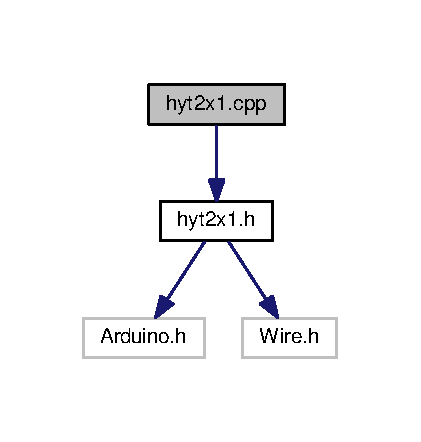
\includegraphics[width=202pt]{hyt2x1_8cpp__incl}
\end{center}
\end{figure}
\subsection*{Namespaces}
\begin{DoxyCompactItemize}
\item 
 \hyperlink{namespaceHyt2X1}{Hyt2\+X1}
\begin{DoxyCompactList}\small\item\em H\+Y\+T2\+X1 namespace. \end{DoxyCompactList}\end{DoxyCompactItemize}
\subsection*{Functions}
\begin{DoxyCompactItemize}
\item 
uint32\+\_\+t \hyperlink{namespaceHyt2X1_a47e38827f637ac58bbcec76c238de87a}{Hyt2\+X1\+::init\+Read} (uint8\+\_\+t address)
\begin{DoxyCompactList}\small\item\em Init sensor read. \end{DoxyCompactList}\item 
bool \hyperlink{namespaceHyt2X1_ab2e26ccda85abca1e0d3f29bd5ea7039}{Hyt2\+X1\+::read} (int8\+\_\+t address, float $\ast$humidity, float $\ast$temperature)
\begin{DoxyCompactList}\small\item\em Returns the humidty and temperature from hyt2\+X1 sensor at specified address. \end{DoxyCompactList}\item 
void \hyperlink{namespaceHyt2X1_a4b974cad973a8aa5b8525c1c5cb85dd7}{Hyt2\+X1\+::send} (int8\+\_\+t address, uint8\+\_\+t data\+\_\+0, uint8\+\_\+t data\+\_\+1, uint8\+\_\+t data\+\_\+2)
\begin{DoxyCompactList}\small\item\em Send sensor command. \end{DoxyCompactList}\item 
void \hyperlink{namespaceHyt2X1_a06824bbb5dc4a87a4cd51249b43ba9c2}{Hyt2\+X1\+::change\+Address} (uint8\+\_\+t power\+\_\+pin, int8\+\_\+t address, int8\+\_\+t new\+\_\+address)
\begin{DoxyCompactList}\small\item\em Change sensor address. \end{DoxyCompactList}\item 
void \hyperlink{namespaceHyt2X1_a128d06772378bc6c052b01094407950c}{Hyt2\+X1\+::init} (uint8\+\_\+t power\+\_\+pin)
\begin{DoxyCompactList}\small\item\em Init sensor. \end{DoxyCompactList}\item 
void \hyperlink{namespaceHyt2X1_a37cb490fe77882a734352359f0c2fba5}{Hyt2\+X1\+::on} (uint8\+\_\+t power\+\_\+pin)
\begin{DoxyCompactList}\small\item\em Power on sensor. \end{DoxyCompactList}\item 
void \hyperlink{namespaceHyt2X1_ae78eebe12bb6a879bc487ec001416b2e}{Hyt2\+X1\+::off} (uint8\+\_\+t power\+\_\+pin)
\begin{DoxyCompactList}\small\item\em Power off sensor. \end{DoxyCompactList}\end{DoxyCompactItemize}

\hypertarget{hyt2x1_8h}{}\section{hyt2x1.\+h File Reference}
\label{hyt2x1_8h}\index{hyt2x1.\+h@{hyt2x1.\+h}}
{\ttfamily \#include \char`\"{}Arduino.\+h\char`\"{}}\newline
{\ttfamily \#include $<$Wire.\+h$>$}\newline
Include dependency graph for hyt2x1.\+h\+:
\nopagebreak
\begin{figure}[H]
\begin{center}
\leavevmode
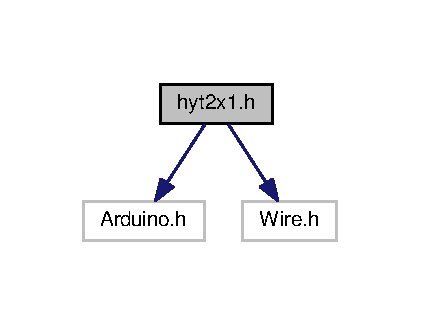
\includegraphics[width=202pt]{hyt2x1_8h__incl}
\end{center}
\end{figure}
This graph shows which files directly or indirectly include this file\+:
\nopagebreak
\begin{figure}[H]
\begin{center}
\leavevmode
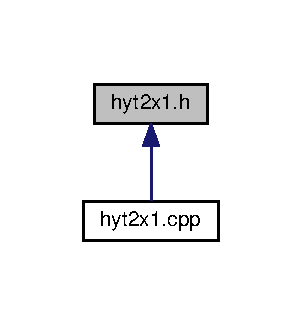
\includegraphics[width=145pt]{hyt2x1_8h__dep__incl}
\end{center}
\end{figure}
\subsection*{Namespaces}
\begin{DoxyCompactItemize}
\item 
 \hyperlink{namespaceHyt2X1}{Hyt2\+X1}
\begin{DoxyCompactList}\small\item\em H\+Y\+T2\+X1 namespace. \end{DoxyCompactList}\end{DoxyCompactItemize}
\subsection*{Macros}
\begin{DoxyCompactItemize}
\item 
\mbox{\Hypertarget{hyt2x1_8h_a120f62242e71b34fb01ca1904fd13112}\label{hyt2x1_8h_a120f62242e71b34fb01ca1904fd13112}} 
\#define \hyperlink{hyt2x1_8h_a120f62242e71b34fb01ca1904fd13112}{H\+Y\+T2\+X1\+\_\+\+D\+E\+F\+A\+U\+L\+T\+\_\+\+A\+D\+D\+R\+E\+SS}~(0x28)
\begin{DoxyCompactList}\small\item\em Default address. \end{DoxyCompactList}\item 
\mbox{\Hypertarget{hyt2x1_8h_a9603babe84e5c9e5ef910a52fca9194f}\label{hyt2x1_8h_a9603babe84e5c9e5ef910a52fca9194f}} 
\#define \hyperlink{hyt2x1_8h_a9603babe84e5c9e5ef910a52fca9194f}{H\+Y\+T2\+X1\+\_\+\+R\+E\+A\+D\+\_\+\+H\+T\+\_\+\+D\+A\+T\+A\+\_\+\+L\+E\+N\+G\+TH}~(4)
\begin{DoxyCompactList}\small\item\em Number of bytes to be read. \end{DoxyCompactList}\item 
\mbox{\Hypertarget{hyt2x1_8h_a20351d7b7f39273a64819751d617e3da}\label{hyt2x1_8h_a20351d7b7f39273a64819751d617e3da}} 
\#define \hyperlink{hyt2x1_8h_a20351d7b7f39273a64819751d617e3da}{H\+Y\+T2\+X1\+\_\+\+E\+N\+T\+E\+R\+\_\+\+C\+O\+M\+M\+A\+N\+D\+\_\+\+M\+O\+DE}~(0x\+A0)
\begin{DoxyCompactList}\small\item\em Command mode. \end{DoxyCompactList}\item 
\mbox{\Hypertarget{hyt2x1_8h_abf498c5fba7c5a501a36698cac1f131b}\label{hyt2x1_8h_abf498c5fba7c5a501a36698cac1f131b}} 
\#define \hyperlink{hyt2x1_8h_abf498c5fba7c5a501a36698cac1f131b}{H\+Y\+T2\+X1\+\_\+\+E\+X\+I\+T\+\_\+\+C\+O\+M\+M\+A\+N\+D\+\_\+\+M\+O\+DE}~(0x80)
\begin{DoxyCompactList}\small\item\em Exit command mode. \end{DoxyCompactList}\item 
\mbox{\Hypertarget{hyt2x1_8h_a836a95d023481badcc84a5f31d9f95a6}\label{hyt2x1_8h_a836a95d023481badcc84a5f31d9f95a6}} 
\#define \hyperlink{hyt2x1_8h_a836a95d023481badcc84a5f31d9f95a6}{H\+Y\+T2\+X1\+\_\+\+W\+R\+I\+T\+E\+\_\+\+A\+D\+D\+R\+E\+SS}~(0x5\+C)
\begin{DoxyCompactList}\small\item\em Write address. \end{DoxyCompactList}\item 
\mbox{\Hypertarget{hyt2x1_8h_ad4162be756170c512c20dea6ccf32a17}\label{hyt2x1_8h_ad4162be756170c512c20dea6ccf32a17}} 
\#define \hyperlink{hyt2x1_8h_ad4162be756170c512c20dea6ccf32a17}{H\+Y\+T2\+X1\+\_\+\+C\+O\+N\+V\+E\+R\+S\+I\+O\+N\+\_\+\+T\+I\+M\+E\+\_\+\+MS}~(100)
\begin{DoxyCompactList}\small\item\em Conversion time in milliseconds. \end{DoxyCompactList}\item 
\mbox{\Hypertarget{hyt2x1_8h_adfc562673f05e37558390033dcb0abc3}\label{hyt2x1_8h_adfc562673f05e37558390033dcb0abc3}} 
\#define \hyperlink{hyt2x1_8h_adfc562673f05e37558390033dcb0abc3}{H\+Y\+T2\+X1\+\_\+\+T\+E\+M\+P\+E\+R\+A\+T\+U\+R\+E\+\_\+\+M\+IN}~(-\/40)
\begin{DoxyCompactList}\small\item\em Minimum temperature. \end{DoxyCompactList}\item 
\mbox{\Hypertarget{hyt2x1_8h_a08f1e6f8f3b56531cfb988ac5e2e4140}\label{hyt2x1_8h_a08f1e6f8f3b56531cfb988ac5e2e4140}} 
\#define \hyperlink{hyt2x1_8h_a08f1e6f8f3b56531cfb988ac5e2e4140}{H\+Y\+T2\+X1\+\_\+\+T\+E\+M\+P\+E\+R\+A\+T\+U\+R\+E\+\_\+\+M\+AX}~(125)
\begin{DoxyCompactList}\small\item\em Maximum temperature. \end{DoxyCompactList}\item 
\mbox{\Hypertarget{hyt2x1_8h_ad131c698960ea1dce05662be6da41a98}\label{hyt2x1_8h_ad131c698960ea1dce05662be6da41a98}} 
\#define \hyperlink{hyt2x1_8h_ad131c698960ea1dce05662be6da41a98}{H\+Y\+T2\+X1\+\_\+\+H\+U\+M\+I\+D\+I\+T\+Y\+\_\+\+M\+IN}~(0)
\begin{DoxyCompactList}\small\item\em Minimum humidity. \end{DoxyCompactList}\item 
\mbox{\Hypertarget{hyt2x1_8h_a662d874ec5045ecb6605319f9ed47d5a}\label{hyt2x1_8h_a662d874ec5045ecb6605319f9ed47d5a}} 
\#define \hyperlink{hyt2x1_8h_a662d874ec5045ecb6605319f9ed47d5a}{H\+Y\+T2\+X1\+\_\+\+H\+U\+M\+I\+D\+I\+T\+Y\+\_\+\+M\+AX}~(100)
\begin{DoxyCompactList}\small\item\em Maximum humidity. \end{DoxyCompactList}\end{DoxyCompactItemize}
\subsection*{Functions}
\begin{DoxyCompactItemize}
\item 
void \hyperlink{namespaceHyt2X1_a128d06772378bc6c052b01094407950c}{Hyt2\+X1\+::init} (uint8\+\_\+t power\+\_\+pin)
\begin{DoxyCompactList}\small\item\em Init sensor. \end{DoxyCompactList}\item 
void \hyperlink{namespaceHyt2X1_a37cb490fe77882a734352359f0c2fba5}{Hyt2\+X1\+::on} (uint8\+\_\+t power\+\_\+pin)
\begin{DoxyCompactList}\small\item\em Power on sensor. \end{DoxyCompactList}\item 
void \hyperlink{namespaceHyt2X1_ae78eebe12bb6a879bc487ec001416b2e}{Hyt2\+X1\+::off} (uint8\+\_\+t power\+\_\+pin)
\begin{DoxyCompactList}\small\item\em Power off sensor. \end{DoxyCompactList}\item 
void \hyperlink{namespaceHyt2X1_a06824bbb5dc4a87a4cd51249b43ba9c2}{Hyt2\+X1\+::change\+Address} (uint8\+\_\+t power\+\_\+pin, int8\+\_\+t address, int8\+\_\+t new\+\_\+address)
\begin{DoxyCompactList}\small\item\em Change sensor address. \end{DoxyCompactList}\item 
uint32\+\_\+t \hyperlink{namespaceHyt2X1_a47e38827f637ac58bbcec76c238de87a}{Hyt2\+X1\+::init\+Read} (uint8\+\_\+t address)
\begin{DoxyCompactList}\small\item\em Init sensor read. \end{DoxyCompactList}\item 
bool \hyperlink{namespaceHyt2X1_ab2e26ccda85abca1e0d3f29bd5ea7039}{Hyt2\+X1\+::read} (int8\+\_\+t address, float $\ast$humidity, float $\ast$temperature)
\begin{DoxyCompactList}\small\item\em Returns the humidty and temperature from hyt2\+X1 sensor at specified address. \end{DoxyCompactList}\item 
void \hyperlink{namespaceHyt2X1_a4b974cad973a8aa5b8525c1c5cb85dd7}{Hyt2\+X1\+::send} (int8\+\_\+t address, uint8\+\_\+t data\+\_\+0, uint8\+\_\+t data\+\_\+1, uint8\+\_\+t data\+\_\+2)
\begin{DoxyCompactList}\small\item\em Send sensor command. \end{DoxyCompactList}\end{DoxyCompactItemize}

%--- End generated contents ---

% Index
\backmatter
\newpage
\phantomsection
\clearemptydoublepage
\addcontentsline{toc}{chapter}{Index}
\printindex

\end{document}
